\documentclass[11pt]{article}
\setlength{\parindent}{0pt}
% page layout
\usepackage[a4paper,margin=1in]{geometry}

% math packages
\usepackage{amsmath,amssymb,amsthm}
\usepackage{mathtools}          % extends amsmath
\usepackage{physics}            % for \dv, \pdv, \ket, etc.
\usepackage{tikz}
\usetikzlibrary{patterns}
\usepackage{enumitem}

% \usepackage{natbib}   
\bibliographystyle{IEEEtran}

% hyperlinks (optional)
\usepackage[colorlinks=true,
linkcolor=blue,     % internal links (e.g. table of contents)
citecolor=blue,     % bibliography citations
urlcolor=blue]{hyperref}

% graphics (optional)
\usepackage{graphicx}

\title{Write Up of Work and Experiments So Far}
\author{Henry}
\date{\today}

\begin{document}

\maketitle

\section{Surface Elevation and Flight Height}

\begin{figure}[hbt]
  \centering
  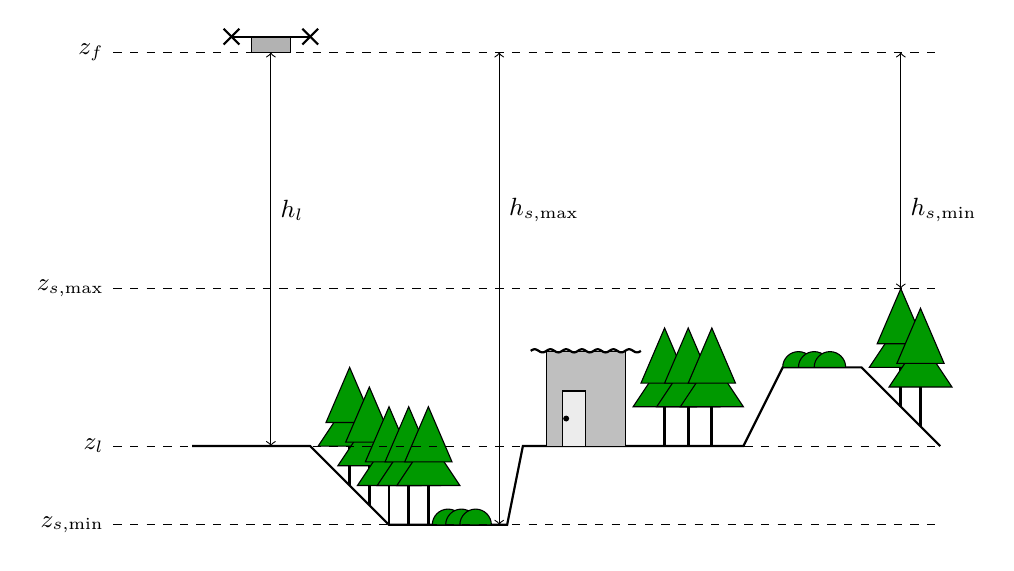
\begin{tikzpicture}[scale=1]
    % Ground profile: uneven terrain
    \draw[thick] 
      (-0.5,0) -- (1,0) -- (2,-1) -- (3.5,-1) -- (3.7,0) -- (5,0) -- (6.5,0) -- (7,1) -- (8,1) -- (9,0);
    % Trees at given (x,y) positions
    \foreach \x/\y in {1.5/0, 1.75/-0.25, 2/-0.5, 2.25/-0.5,2.5/-0.5, 5.5/0.5,5.8/0.5,6.1/0.5, 8.5/1, 8.75/0.75} {
      \draw[line width=1pt] (\x,\y) -- (\x,\y-0.5); % trunk
      % Pine-tree foliage (upright)
      \draw[fill=green!60!black] (\x-0.4,\y) -- (\x+0.4,\y) -- (\x,\y+0.6) -- cycle;
      % Second foliage layer
      \draw[fill=green!60!black] (\x-0.3,\y+0.3) -- (\x+0.3,\y+0.3) -- (\x,\y+1.0) -- cycle;
    }
    % Shrubs at given (x,y) positions
    \foreach \x/\y in {2.75/-1, 2.92/-1, 3.1/-1, 7.2/1, 7.4/1, 7.6/1} {
      % Semi-circular shrub
      \draw[fill=green!60!black] (\x-0.2,\y) arc[start angle=180, end angle=0, radius=0.2] -- (\x+0.2,\y) -- cycle;
    }
    % Building
    \draw[fill=gray!50] (4,0) rectangle (5,1.2);
    \draw[fill=gray!15] (4.2,0) rectangle (4.5, 0.7);
    % Door knob
    \draw[fill=black] (4.25,0.35) circle (0.03);
    % Corrugated-iron roof detail (entirely above top of rectangle)
    \draw[thick, domain=3.8:5.2, samples=100] plot (\x, {1.21 + 0.02*sin(360*5*(\x-4))});
    %\draw (4,1.2) -- (4.5,1.6) -- (5,1.2); % roof
    
    %Elevations
    %Launch
    \draw[dashed, black] (-1.5,0) node[left] {\small $z_{l}$} -- (9,0) ;
    %Max
    \draw[dashed, black] (-1.5,2) node[left] {\small $z_{s,\max}$} -- (9,2);
    %min
    \draw[dashed, black] (-1.5,-1) node[left] {\small $z_{s,\min}$} -- (9,-1);   
    %Flight
    \draw[dashed, black] (-1.5,5) node[left] {\small $z_f$} -- (9,5);
    
    %Heights
    %Launch Height
    \draw[<->, black] (0.5,0) -- (0.5,5);
    %Max Height
    \draw[<->, black] (3.4,-1) -- (3.4,5);
    %Min Height
    \draw[<->, black] (8.5,2) -- (8.5,5);

    % Aligned height labels
    \node[anchor=west] at (0.5,3)   {\small $h_l$};
    \node[anchor=west] at (3.4,3)   {\small $h_{s,\max}$};
    \node[anchor=west] at (8.5,3)   {\small $h_{s,\min}$};

    %Drone
    % UAV icon: rectangle body with two X “propellers”
    \draw[fill=gray!60] (0.25,5) rectangle (0.75,5.2);  % main body centered at (2,2)
    \draw[thick] (0, 5.2) -- (1,5.2);
    \foreach \cx/\y in {0/5.2,1/5.2} {                        % propellers at left/right
    \draw[thick] (\cx-0.1,\y-0.1) -- (\cx+0.1,\y+0.1);
    \draw[thick] (\cx-0.1,\y+0.1) -- (\cx+0.1,\y-0.1);
    }
  \end{tikzpicture}
  \caption{Schematic illustration of uneven terrain with ground features and flight height.}
  \label{fig:SurfaceElevation}
\end{figure}

\noindent
Figure \ref{fig:SurfaceElevation} shows a terrain cross section over an area of interest (AOI), annotated with both absolute elevations (relative to the Australian Height Datum, AHD) and the corresponding UAV flight heights above ground.\\


\noindent
In this schematic, the solid line depicts the true ground surface profile, including dips and peaks as captured by a Digital Elevation Model (DEM). The overlaid symbols for trees, shrubs, and the building represent above-ground features that together constitute a Digital Surface Model (DSM).\\

\noindent
Absolute elevations denoted by $z$ mark key points relative to the Australian Height Datum (AHD). 

\begin{itemize}[label={}]
    \item $z_l$: the elevation at the launch point.
    \item $z_f$: the elevation of the UAV's sensor while in flight, assumed to be constant across AOI.
    \item $z_{s,(x,y)}$: the elevation of the surface at point $(x,y)$.
    \item $z_{s,\min}$: the minimum surface elevation.
    \item $z_{s,\max}$: the maximum surface elevation.
\end{itemize}

Heights denoted by $h$ mark the relative distance between the UAV sensor and the surface. 

\begin{itemize}[label={}]
    \item $h_l = z_f - z_l$, is the flight height at take off. It generally the value given to a flight planner.
    \item $h_{s,(x,y)} = z_f - z_{s,(x,y)}$, is the distance between the UAV and and surface point $(x,y)$.
    \item $h_{s,max} = z_f - z_{s,min}$, is the maximum distance between the UAV and the surface within the AOI.
    \item $h_{s,min} = z_f - z_{s,max}$, is the minimum distance between the UAV and the surface within the AOI.
\end{itemize}

\begin{table}[hbt]
  \centering
  \begin{tabular}{ll}
    \hline
    \textbf{Symbol} & \textbf{Definition} \\
    \hline
    $z_l$            & Launch elevation (AHD) \\
    $z_{s,\max}$     & Maximum surface elevation (AHD) \\
    $z_{s,\min}$     & Minimum surface elevation (AHD) \\
    $z_f$            & Flight elevation (AHD) \\
    $z_{s,(x,y)}$    & Surface elevation at point $(x,y)$ (AHD) \\
    $h_l$            & Flight height above launch ground \\
    $h_{s,(x,y)}$    & Flight height above surface at point $(x,y)$ \\
    $h_{s,\max}$     & Height above highest terrain point \\
    $h_{s,\min}$     & Height above lowest terrain point \\
    \hline
  \end{tabular}
  \caption{Nomenclature of symbols used in this thesis.}
  \label{tab:ElevationNomenclature}
\end{table}

\section{Constraints}
\label{sec:FlightHeight}

\subsection{Pixel Resolution}

The GSD acheived flying at $h_{s,(x,y)}$ is,

\begin{align}
    GSD_{(x,y)} &= \frac{S_x}{f \cdot S_a} \cdot h_{s,(x,y)} \cite{rothPhenoFlyPlanningTool2018}\\
    h_{s,(x,y)} &= \frac{GSD_{(x,y)} \cdot f \cdot S_a}{S_x} \\
    &= \frac{GSD_{(x,y)} \cdot f }{S_\delta}
\end{align}

\noindent
To guareantee that the ground smapling distance at any point $GSD_{(x,y)}$ does not exceed the maximum alowable ground sampling distance $GSD_{req}$:

\begin{align}
    h_{s,max} &\leq \frac{GSD_{req} \cdot f }{S_\delta}\\
    z_f - z_{s,min} &\leq \frac{GSD_{req} \cdot f }{S_\delta}\\
    h_l + z_l - z_{s,min} &\leq \frac{GSD_{req} \cdot f }{S_\delta}\\
    h_l &\leq \frac{GSD_{req} \cdot f }{S_\delta} + z_{s,min} - z_l
\end{align}
\subsection{Diffraction Resolution}

Diffraction preamble...\\

\noindent
Given the diameter of the Airy disk projected to the surface at any point $d_{A,proj,(x,y)}$ must meet the minimum resolution requirement:

\begin{align}
    d_{A,proj,(x,y)} &\leq GSD_{req}\\
    d_{A} \cdot \frac{h_{s,(x,y)}}{f} &\leq GSD_{req}\\
    \frac{2.44 \cdot N \cdot \lambda \cdot h_{s,(x,y)}}{f} &\leq GSD_{req}\\
    h_{s,(x,y)} &\leq \frac{GSD_{req} \cdot f}{2.44 \cdot N \cdot \lambda}
\end{align}

\noindent
Again, to guareantee the Airy disk diameter does not exceed the GSD requirement at any point:

\begin{align}
    h_{s,max} &\leq \frac{GSD_{req} \cdot f}{2.44 \cdot N \cdot \lambda}\\
    z_f - z_{s,min} &\leq \frac{GSD_{req} \cdot f}{2.44 \cdot N \cdot \lambda}\\
    h_l + z_l - z_{s,min} &\leq \frac{GSD_{req} \cdot f}{2.44 \cdot N \cdot \lambda}\\
    h_l &\leq \frac{GSD_{req} \cdot f}{2.44 \cdot N \cdot \lambda} + z_{s,min} - z_l
\end{align}

\subsection{Depth of Field}

\begin{figure}[hbt]
  \centering
  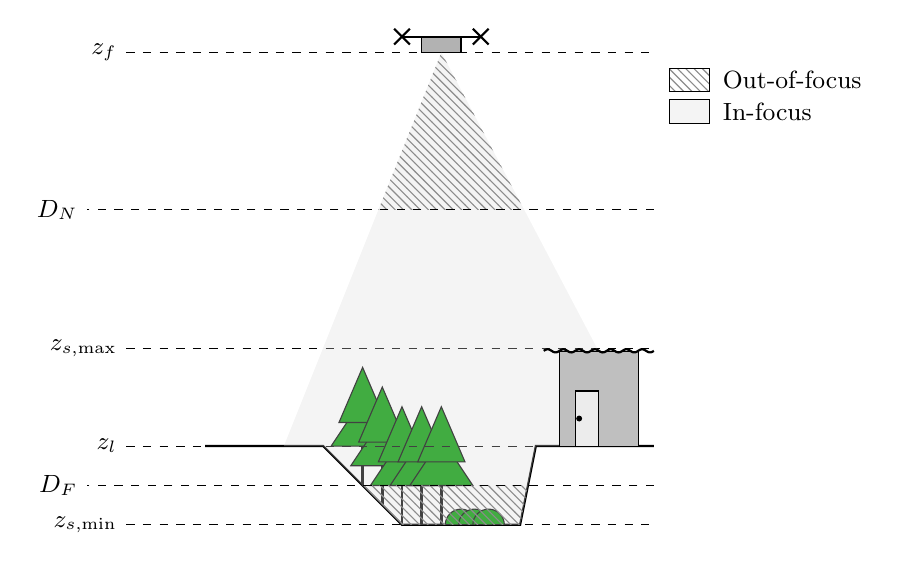
\begin{tikzpicture}[scale=1]
    % Ground profile: uneven terrain (cropped at x=5.2)
    \draw[thick] 
      (-0.5,0) -- (1,0) -- (2,-1) -- (3.5,-1) -- (3.7,0) -- (5,0) -- (5.2,0);
    % Trees at given (x,y) positions, only for x ≤ 5.2
    \foreach \x/\y in {1.5/0, 1.75/-0.25, 2/-0.5, 2.25/-0.5, 2.5/-0.5} {
      \draw[line width=1pt] (\x,\y) -- (\x,\y-0.5); % trunk
      % Pine-tree foliage (upright)
      \draw[fill=green!60!black] (\x-0.4,\y) -- (\x+0.4,\y) -- (\x,\y+0.6) -- cycle;
      % Second foliage layer
      \draw[fill=green!60!black] (\x-0.3,\y+0.3) -- (\x+0.3,\y+0.3) -- (\x,\y+1.0) -- cycle;
    }
    % Shrubs at given (x,y) positions, only for x ≤ 5.2
    \foreach \x/\y in {2.75/-1, 2.92/-1, 3.1/-1} {
      % Semi-circular shrub
      \draw[fill=green!60!black] (\x-0.2,\y) arc[start angle=180, end angle=0, radius=0.2] -- (\x+0.2,\y) -- cycle;
    }
    

    % Elevations (dashed lines, cropped at x=5.2)
    % Launch
    \draw[dashed, black] (-1.5,0) node[left] {\small $z_{l}$} -- (5.2,0) ;
    % Max surface
    \draw[dashed, black] (-1.5,1.24) node[left] {\small $z_{s,\max}$} -- (5.2,1.24);
    % Min surface
    \draw[dashed, black] (-1.5,-1) node[left] {\small $z_{s,\min}$} -- (5.2,-1);   
    % Flight
    \draw[dashed, black] (-1.5,5) node[left] {\small $z_f$} -- (5.2,5);

    % % Heights (arrows, third arrow at x=5.2)
    % % Launch Height
    % \draw[<->, black] (0.5,0) -- (0.5,5);
    % % Max Height
    % \draw[<->, black] (3.4,-1) -- (3.4,5);
    % % Min Height (cropped at x=5.2)
    % \draw[<->, black] (5.2,1.5) -- (5.2,5);

    % % Aligned height labels at y=3 along their respective x-tip values
    % \node[anchor=west] at (0.5,3)   {\small $h_l$};
    % \node[anchor=west] at (3.4,3)   {\small $h_{s,\max}$};
    % \node[anchor=west] at (5.2,3)   {\small $h_{s,\min}$};

    % Drone (UAV icon centered at x=2.5)
    \draw[fill=gray!60] (2.25,5) rectangle (2.75,5.2);  % body centered at x=2.5
    \draw[thick] (2.0,5.2) -- (3.0,5.2);                % propeller bar
    \foreach \cx/\y in {2.0/5.2,3.0/5.2} {              % propellers at left/right
      \draw[thick] (\cx-0.1,\y-0.1) -- (\cx+0.1,\y+0.1);
      \draw[thick] (\cx-0.1,\y+0.1) -- (\cx+0.1,\y-0.1);
    }
    % Cone of view from UAV to surface points (fill only, no outline)
    \fill[gray!30, opacity=0.3] 
      (2.5,5) -- (0.5,0) -- (1,0) -- (2,-1) -- (3.5,-1) -- (3.7,0) -- (4.5,0) -- (4.5,1.2) -- cycle;
    
      % Striped pattern on cone top region (y ≥ 3.5)
    \begin{scope}
      \clip (2.5,5) -- (0.5,0) -- (4.5,1.2) -- cycle;  % cone shape
      \clip (-1,3) rectangle (6,5.5);
      \fill[pattern=north west lines, pattern color=gray!90] (-1,3) rectangle (6,5.5);
    \end{scope}

    % Striped pattern on cone bottom region (y ∈ [−1,−0.5])
    \begin{scope}
      \clip (2.5,5) -- (0.5,0) -- (1,0) -- (2,-1) -- (3.5,-1) -- (3.7,0) -- (4.5,0) -- (4.5,1.2) -- cycle;  % full cone polygon
      \clip (-1,-1) rectangle (6,-0.5);
      \fill[pattern=north west lines, pattern color=gray!90] (-1,-1) rectangle (6,-0.5);
    \end{scope}

    % DOF Lines aligned with elevations on left of cone
    \draw[dashed,black] (5.2,3) -- (-2,3) node[left] {\small $D_N$};
    \draw[dashed,black] (5.2,-0.5) -- (-2,-0.5) node[left] {\small $D_F$};
    
    \begin{scope}
    \draw[pattern=north west lines, pattern color=gray!90] (5.4,4.5) rectangle +(0.5,0.3);
    \node[anchor=west] at (5.95,4.65) {\small Out-of-focus};
    \end{scope}
    % Legend: in-focus field of view (gray region), just below previous
    \begin{scope}
    \fill[gray!30, opacity=0.3] (5.4,4.1) rectangle +(0.5,0.3);
    \draw (5.4,4.1) rectangle +(0.5,0.3);
    \node[anchor=west] at (5.95,4.25) {\small In-focus};
    \end{scope}

    % Building (rightmost x=5 ≤ 5.2, so keep as-is)
    \draw[fill=gray!50] (4,0) rectangle (5,1.2);
    \draw[fill=gray!15] (4.2,0) rectangle (4.5, 0.7);
    % Door knob
    \draw[fill=black] (4.25,0.35) circle (0.03);
    % Corrugated-iron roof detail
    \draw[thick, domain=3.8:5.2, samples=100] plot (\x, {1.21 + 0.02*sin(360*5*(\x-4))});

  \end{tikzpicture}
  \caption{Near and far limits to a UAV mounted sensor's field of view. Shrubs at the bottom of the gully fall beyond the far limit and are thus considerd out of focus.}
  \label{fig:DOF1}
\end{figure}

\noindent
The near limit $D_N$ and far limit $D_F$ denote the distances along the optical axis from the sensor plane (or camera's principal plane) to the near and far focus limits, respectively.

\begin{align}
    D_N &= \frac{s\cdot H}{H + s} \cite{rothPhenoFlyPlanningTool2018}\\
    D_F &= \frac{s\cdot H}{H - s} \cite{rothPhenoFlyPlanningTool2018} \label{eq:dof_far}\\ 
\end{align}

\noindent 
where $s$ is the set focus distance and $H$ is the Hyperfocal distance of the sensor:

\begin{align}
    H &= \frac{f^2}{N \cdot c} + f \label{eq:hyperfocal} \cite{rothPhenoFlyPlanningTool2018}
\end{align}

\noindent
While most imaging systems support adjustable focus distances, it is reasonable to assume a fixed focus distance for drone-based photogrammetry. In typical deployments, the camera is calibrated once prior to operation, and the focus is then locked. Recalibrating before every flight is inefficient and often impractical, particularly for fully autonomous systems. Maintaining a constant focus distance ensures that internal camera parameters, such as focal length and distortion coefficients, remain valid across missions, ensuring reliable and repeatable data capture without the need for continual recalibration \cite{luhmannSensorModellingCamera2016}.\\

\noindent
Equation \ref{eq:dof_far} indicates as $s$ approaches $H$ from below, $D_F$ tends to infinity; if $s$ exceeds $H$, the denominator becomes negative, yielding a non-physical negative far limit. To ensure a real, non-negative focus range, the focus distance must satisfy, 

\begin{align}
  s &\leq H
\end{align}

\noindent
To ensure the entire surface is captured in focus by the sensor, launch height must be adjusted such that the minimum and maxium elevations fall within the near and far limits to the DOF.

\begin{align}
    D_N &\leq z_f - z_{s,\max}\\
    D_N &\leq z_l + h_l - z_{s,\max}\\
    h_l &\geq D_N + z_{s,\max} - z_l\\
    h_l &\geq \frac{s\cdot H}{H + s} + z_{s,\max} - z_l\\
    h_l &\geq \frac{N \cdot c \cdot f \cdot s + s \cdot f^2}{N \cdot c \cdot (f+s) + f^2} + z_{s,\max} - z_l \label{eq:hD_N}
\end{align}

\begin{align}
    D_F &\geq z_f - z_{s,\min}\\
    D_F &\geq z_l + h_l - z_{s,\min}\\
    h_l &\leq D_F + z_{s,\min} - z_l\\
    h_l &\leq \frac{s\cdot H}{H - s} + z_{s,\min} - z_l\\
    h_l &\leq \frac{N \cdot c \cdot f \cdot s + s \cdot f^2}{N \cdot c \cdot (f-s) + f^2} + z_{s,\min} - z_l \label{eq:hD_F}
\end{align}

\noindent
Figure \ref{fig:DOF1} shows a scene where launch height meets \ref{eq:hD_N} but not \ref{eq:hD_F} resulting in shrubery in the gully being captured out of focus. 

\subsection{Motion Blur}

Motion blur preamble... \\

\noindent
Motion blur $\delta$ meausred in pixels, can be estimated at any point $(x,y)$ in the direction of flight as,

\begin{align}
    \delta &= \frac{v_{(x,y)} \cdot I_t}{GSD_{(x,y)}} \cite{oconnorCamerasSettingsAerial2017b}
\end{align}

\noindent
Assuming the linear velocity remains constant across the AOI, it must be selected such that motion blur is less than a given maximum $\delta_{\max}$ at all points. 

\begin{align}
    v &\leq \frac{GSD_{(x,y)} \cdot \delta_{\max}}{I_t} 
\end{align}

\noindent
Given,

\begin{align}
    GSD_{\min} &= \frac{S_\delta}{f} \cdot h_{s,(\min)}
\end{align}

\noindent
Velocity must be selected such that,

\begin{align}
    v &\leq \frac{ S_\delta \cdot h_{s,(\min)} \cdot \delta_{\max}}{f \cdot I_t} \\
    v &\leq \frac{ S_\delta \cdot (z_f - z_{s,\max}) \cdot \delta_{\max}}{f \cdot I_t} \\
    v &\leq \frac{ S_\delta \cdot (h_l + z_l - z_{s,\max}) \cdot \delta_{\max}}{f \cdot I_t}
\end{align}

or height must be selected such that,
\begin{align}
  h_l \geq \frac{v\cdot f\cdot I_t}{S_\delta \cdot \delta_{\max}} - z_l + z_{s,\max}
\end{align}

However, the selected exposure time $I_t$ is tied to the required exposure value,
\begin{align}
  EV = \log_2(\frac{N^2}{I_t}) + \log_2(\frac{100}{ISO}) \label{eq:ExposureVal}
\end{align}
and can thus be expressed in terms of aperture if we assume ISO is fixed at its maximum ($ISO_{\max})$,
\begin{align}
  I_t = \frac{100\cdot N^2}{2^{EV} \cdot ISO_{\max}}
\end{align}
Hence,
\begin{align}
  h_l \geq \frac{ 100 \cdot N^2 \cdot v \cdot f}{2^{EV} \cdot ISO_{\max} \cdot S_\delta \cdot \delta_{\max}} - z_l + z_{s,\max}
\end{align}

\subsection{End Overlap}

Endlap preamble....

  \begin{figure}[hbt]
    \centering
    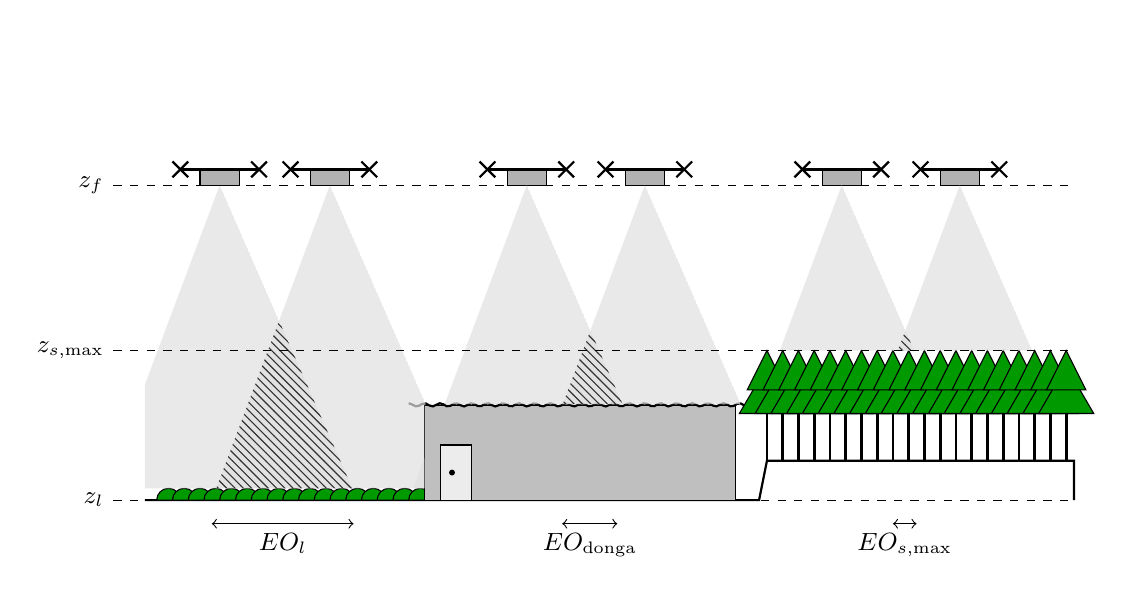
\begin{tikzpicture}[scale=1]
      % Ground baseline
      \draw[thick] (-1.3,0) -- (6.5,0) -- (6.6,0.5) -- (10.5,0.5) -- (10.5,0);

      %% Segment 1: (removed explicit drones/cones)
      % Shrubs
      \foreach \x in {-1,-0.8,-0.6,-0.4,-0.2,0,0.2,0.4,0.6,0.8,1,1.2,1.4,1.6,1.8,2,2.2,2.4,2.6,2.8,3,3.2,3.4} {
        \draw[fill=green!60!black] (\x-0.15,0) arc[start angle=180,end angle=0,radius=0.15] 
          -- (\x+0.15,0) -- cycle;
      }

      %% Segment 1.5: Wide building between shrubs and trees
      % Building
      \draw[fill=gray!50] (2.25,0) rectangle (6.2,1.2);
      \draw[fill=gray!15] (2.45,0) rectangle (2.85,0.7);
      \draw[fill=black] (2.6,0.35) circle (0.03);
      % Corrugated-iron roof detail
      \draw[thick, domain=2.05:6.4, samples=100] plot(\x, {1.21 + 0.02*sin(360*5*(\x-3))});

      %% Segment 2: (removed explicit drones/cones)

      % Trees
      \foreach \x in {6.6,6.8,7,7.2,7.4,7.6,7.8,8,8.2,8.4,8.6,8.8,9,9.2,9.4,9.6,9.8,10,10.2,10.4} {
        \draw[line width=1pt] (\x,0.5) -- (\x,1.1);
        \draw[fill=green!60!black] (\x-0.35,1.1) -- (\x+0.35,1.1) -- (\x,1.7) -- cycle;
        \draw[fill=green!60!black] (\x-0.25,1.4) -- (\x+0.25,1.4) -- (\x,1.9) -- cycle;
      }

      %% Segment 3: (removed explicit drones/cones)

      % ---------- Drones and cones (clipped to surface) ----------
      \foreach \idx/\Cx/\Ybot in {
        0/ -0.1/0, 1/ 1.3/0,
        2/ 3.8/0, 3/ 5.3/0,
        4/ 7.8/0, 5/ 9.3/0
      }{
        % Drone (unchanged)
        \draw[fill=gray!60] (\Cx-0.5,4) rectangle (\Cx,4.2);
        \draw[thick] (\Cx-0.75,4.2) -- (\Cx+0.25,4.2);
        \foreach \dx in {\Cx-0.75,\Cx+0.25} {
          \draw[thick] (\dx-0.1,4.1) -- (\dx+0.1,4.3);
          \draw[thick] (\dx-0.1,4.3) -- (\dx+0.1,4.1);
        }
        % Cone clipped above surface/profile
        \begin{scope}
          % Clip everything below the ground profile ADJUSTED X
          \clip (-1.3,0.15) -- (2.25,0.15) -- (2.25,1.22) -- (6.3,1.22) -- (6.3,1.9) -- (10.5,1.9)
                -- (10.5,6) -- (-1.3,6) -- cycle;
          % Clip to this cone’s triangle
          \clip (\Cx-0.25,4) -- (\Cx-1.75,\Ybot) -- (\Cx+1.5,\Ybot) -- cycle;
          % Fill the clipped cone
          \fill[gray!25, opacity=0.7]
            (\Cx-0.25,4) -- (\Cx-1.75,\Ybot) -- (\Cx+1.5,\Ybot) -- cycle;
        \end{scope}
      }

      % ---------- Stripe only the overlaps between each adjacent cone pair ----------
      \foreach \Cfirst/\Csecond/\Yb in {
        -0.1/1.3/0,  3.8/5.3/0,  7.8/9.3/0
      }{
        \begin{scope}
          % Clip below ground
          \clip (-1.3,0.15) -- (2.25,0.15) -- (2.25,1.22) -- (6.3,1.22) -- (6.3,1.9) -- (10.5,1.9)
                -- (10.5,6) -- (-1.3,6) -- cycle;
          % Clip to first cone
          \clip (\Cfirst-0.25,4) -- (\Cfirst-1.75,\Yb)
                -- (\Cfirst+1.5,\Yb) -- cycle;
          % Clip to second cone
          \clip (\Csecond-0.25,4) -- (\Csecond-1.75,\Yb)
                -- (\Csecond+1.5,\Yb) -- cycle;
          % Fill intersection with stripes
          \fill[pattern=north west lines, pattern color=black!80]
            (\Csecond-1.75,\Yb) rectangle (\Cfirst+1.5,4);
        \end{scope}
      }
      % ---------- Elevation reference lines ----------
      \draw[dashed,black] (-1.7,0)    node[left] {\small $z_l$}        -- (10.5,0);
      \draw[dashed,black] (-1.7,1.9)  node[left] {\small $z_{s,\max}$} -- (10.5,1.9);
      \draw[dashed,black] (-1.7,4)  node[left] {\small $z_f$}        -- (10.5,4);

      % ---------- End-overlap arrows along X axis ----------
      % First pair overlap arrow
      \draw[<->] (-0.45,-0.3) -- (1.35,-0.3) node[midway,below] {\small $EO_{l}$};
      % Second pair overlap arrow
      \draw[<->] (4,-0.3) -- (4.7,-0.3) node[midway,below] {\small $EO_{\text{donga}}$};
      % Third pair overlap arrow
      \draw[<->] (8.2,-0.3) -- (8.5,-0.3) node[midway,below] {\small $EO_{s,\max}$};
    \end{tikzpicture}
    \caption{End overlaps at differnt surface hights. With a constant flight elevation, the end overlap $EO_{s,\max}$ when the surface elevation is at its maximum, is less than the overlap at launch $EO_l$.}
    \label{fig:EndOverlap}
  \end{figure}

\noindent
Given a minimum required percentage overlap between sucessive images $EO_{req}$, the neccasary ground spacing between image captures at any point $E_{(x,y)}$ is,

\begin{align}
    E_{(x,y)} &= G_E \cdot (1-\frac{EO_{req}}{100}) \cite{rothPhenoFlyPlanningTool2018}
\end{align}
\noindent
where $G_E$ is the ground field of view in the direction of flight. Assuming the sensor is orientated such that the y axis is paralell to the direction of flight\footnote{Orientating the wider $x$ axis of the sensor perpendicular to the flight direction, increases the area covered by each flight line. This minimises flight time as less turns are required to cover the same area.}, 
\begin{align}
    E_{(x,y)} &= \frac{S_y}{f} \cdot h_{s,(x,y)} \cdot (1-\frac{EO_{req}}{100})
\end{align}



\noindent
As the minimum end overlap will occur at $h_{s,min}$ as illistrated in Figure \ref{fig:EndOverlap}, 

\begin{align}
    E_{\max} &= \frac{S_y}{f} \cdot h_{s,\min} \cdot (1-\frac{EO_{req}}{100})\\
    &= \frac{S_y}{f} \cdot (h_l + z_l - z_{s,max}) \cdot (1-\frac{EO_{req}}{100})\\
\end{align}

\noindent
Thus, velocity must be selected such that,

\begin{align}
   v &\leq I_{f,\max} \cdot E_{\max}\\
   v &\leq I_{f,\max} \cdot \frac{S_y}{f} \cdot (h_l + z_l - z_{s,max}) \cdot (1-\frac{EO_{req}}{100})
\end{align}

or height must be selected such that,
\begin{align}
  h_l \geq \frac{v \cdot f}{I_{f,\max} \cdot S_y \cdot (1-\frac{EO_{req}}{100})} - z_l + z_{s,max}
\end{align}

\noindent
where $I_{f,\max}$ is the maximum capture freqency of the imaging system. 

\subsection{Constant Constraints}
Legal and Physical

\newpage
\section{Optimization}

\subsection{Objective}
Objective preamble about coverage removing flight path from consideration etc\dots\\

The coverage rate can be defined as the area covered by the sensors field of view every second. 
\begin{align}
  F(h,v) &= \frac{S_x}{f} \cdot h \cdot v \label{eq:ObjFunc}
\end{align}

\subsection{Solution Space}

\textbf{Present the solution space for a few examples and explain why a optimiser is required.}\\

% Given the constraints on launch height and linear velocity derived in Sections \ref{sec:FlightHeight} and \ref{sec:Velocity}, and the sensor specific variables and constraints on aperture, exposure time and sensor sensitivity, determining the optimal set of these parameters can be difficult to do by hand. \\

% This complexity is particularly pronounced in scenarios where optimal solutions are non-intuitive. For instance, if a UAV’s fixed focus distance is sub-optimal for a given task, the upper limit on allowable flight height shifts from being constrained primarily by the ground sampling distance (GSD) to the far limit of the depth-of-field (DOF). Such constraints, which are less intuitive to operators, significantly complicate decision-making.\\

% Furthermore, in applications demanding low sensor noise where ISO sensitivity is strictly limited, the interplay between aperture settings, exposure time, and exposure value (EV) yields an irregular, and often non-intuitive feasible region. As a result, a systematic optimization method is necessary to ensure reliable, consistent, and optimal flight parameter selection.



\subsection{Problem Formulation}

Rather than attempting to search the full three-dimensional space \((h,v,N)\) simultaneously, we can exploit the fact that sensor apertures are constrained to a discrete set of stops $\mathcal{N} = \{N_1,N_2,...,N_n\}$. This means we can slice the 3D solution space into $n$ 2D spaces and compare the optimal height and velocity for each $N \in \mathcal{N}$. \\

Thus, for a fixed aperture, each upper bound $u_i(v;N) \in \mathcal{U}$ and lower bound $l_j(v;N) \in \mathcal{L}$ on height derived in Section \ref{sec:FlightHeight} is affine in $(v,h)$, 
\begin{align}
  h &\leq m_i(N)v + b_i(N) \quad \forall i \in \mathcal{U}\\
  h &\geq \bar{m_j}(N)v + \bar{b_j}(N) \quad \forall j \in \mathcal{L}
\end{align}

As each upper bound is linear, their pointwise minimum,
\begin{align}
  h_{\max}(v;N) &= \min_{i \in \mathcal{U}}\{m_i(N)v + b_i(N)\}
\end{align}
is a concave piecewise linear surface in the $(v,h)$ plane. A feasible $(v,h)$ must lie at or below this surface. Similarly, all feasible $(v,h)$ must lie at or above the convex peicewise linear surface of linear lower bounds,
\begin{align}
  h_{\min}(v;N) &= \max_{j \in \mathcal{L}}\{\bar{m_j}(N)v + \bar{b_j}(N)\}
\end{align}

As the objective function \ref{eq:ObjFunc} is monotonically increasing in $h$, the optimal height at a fixed velocity and aperture will always lie on the upper bound. That is,
\begin{align}
  h(v;N)^* &= h_{\max}(v;N), \quad \forall \; v \in [v_{\min},v_{\max}]
\end{align}

This collapses the problem into a one dimentional optimisation over velocity,
\begin{align}
  \max_{v\in[v_{\min},v_{\max}]}\;F(v;N) \label{eq:oneDobjmax}
\end{align}
where,
\begin{align}
  F(v;N) &= \frac{S_x}{f} \cdot h_{\max}(v,N) \cdot v \label{eq:oneDobj}
\end{align}


\subsection{Vertex Enumeration Justification}

Within a given segment $I_i$ the objective \ref{eq:oneDobj} becomes quadratic,
\begin{align}
    F(v;N) = \frac{S_x}{f}(m_i(N)v^2 + b_i(N)v)
\end{align}
and the local maximum can only occur at two points.
\begin{enumerate}
  \item If $m_i(N) \geq 0$, $F(v;N)$ is linear or stricly convex in $v$. In both cases the local maximum occurs at the right end point of the segment.
  \item If $m_i(N) < 0$, $F(v;N)$ is stricly concave and a local maximum can occur at the stationary point where $\frac{\partial F}{\partial v} = 0$,
  \begin{align}
    \hat{v_i} = -\frac{b_i(N)}{2\,m_i(N)}
  \end{align} which, provided it lies inside $I_i$ and satisfies the floor constraint, is a local maximum. If $\hat{v_i} $ is infeasible or outside the segment, again the right endpoint is best.
\end{enumerate}

Hence, the global maximiser of the one-dimensional problem \ref{eq:oneDobjmax} must occur at a breakpoint of $h_{\max}(v;N)$, at the domain endpoints or, in the case that $m_i(N) < 0$, at a stationary point $\hat{v_i}$.\\

However, the upper bounds derived in Section \ref{sec:FlightHeight} are constant in $(v,h)$. Therefore all $m_i(N) = 0$, the objective function \ref{eq:oneDobj} is linear in $v$ and we can ignore the stationary point $\hat{v_i}$. \\
% \begin{align}
%     \mathcal V(N)
%   &= \{\,v_{\min},\,v_{\max}\}\\
%     &\;\cup\;
%     \bigl\{\,v\in[v_{\min},v_{\max}]\;\bigm|\;
%       u_i(v;N)=u_k(v;N),\;i<k
%     \bigr\}\\
%     &\;\cup\;
%     \bigl\{\,v\in[v_{\min},v_{\max}]\;\bigm|\;
%       u_i(v;N)=\ell_j(v;N),\;i\in\mathcal U,\;j\in\mathcal L
%     \bigr\}.
% \end{align}

This follows the fundemental theorem in linear optimisation; if a linear program has an optimal solution, then at least one optimal solution occurs at a vertex (an extreme point) of its feasible polytope \cite{bertsimasIntroductionLinearOptimization1997}. In our setting the “polytope” in the $(v,h)$ plane is defined by the peicewise linear functions, $h_{\max}(v;N)$ and $h_{\min}(v;N)$.\\


By restricting our search to this finite set of velocities, we avoid any need for iterative solvers or numerical gradients. The method is both \emph{exact} (no risk of local optima) and \emph{efficient} (only $n$ evaluations for $n$ breakpoints), compared with a generic LP or nonlinear solver that would introduce unnecessary overhead or reliance on convergence tolerances.

\subsection{Vertex Enumeration Algorithm}

To identify the true breakpoints of the concave envelope $h_{\max}(v;N)$, we start by computing two candidate sets:
\begin{align}
  \mathcal{I}_{u,u} = \bigl\{\,v\in[v_{\min},v_{\max}]\;\bigm|\;\exists\;i,k\in\mathcal U,\;i<k:\;u_i(v;N)=u_k(v;N)\bigr\}
\end{align}
and 
\begin{align}
  \mathcal I_{u,\ell} = \bigl\{\,v\in[v_{\min},v_{\max}]\;\bigm|\;\exists\,i\in\mathcal U,\;\exists\,j\in\mathcal L:\;u_i(v;N)=\ell_j(v;N)\bigr\}
\end{align}

However, not every intersection in these sets is a genuine vertex of the feasible ploytope:
\begin{itemize}
  \item Redundant kinks: if the same segment of $h_{\max}(v;N)$ remains active immediately before and after the intersection, $v$ is not an endpoint of the segment and cannot be a local maximum. 
  \item Infeasible points: if at $v$ the active ceiling lies below the floor $(h_{\max}(v;N)<h_{\min}(v;N))$, no valid flight height exists at this velocity.
\end{itemize}

We therefore prune from $\mathcal I_{u,u} \cup \mathcal I_{u,\ell}$, any velocity satisfying either condition. Finally, we add back the domain endpoints $v_{\min}$ and $v_{\max}$ (if they are feasible). The resulting set of velocities $\mathcal{V}(N)$ will contain the optimal velocity for a given aperture.\\

For each aperture N in our discrete set $\mathcal N$, we then evaluate the objective function
\begin{align}
  F(v;N)\;=\;\frac{S_x}{f}\,v\,h_{\max}(v;N), \quad \forall \; v\in\mathcal V(N)
\end{align}
and record the parameters $(v,h)$ yielding the largest $F(v;N)$. Once we have done this for every aperture, we compare the best rates $\{F^*(N)\mid N\in\mathcal N\}$ and select the aperture $N^*$ with the highest mapping speed. The corresponding configuration
\begin{align}
  \bigl(v^*,h^*,N^*\bigr)
\end{align}
is guaranteed to be the global optimum.





















\newpage
\subsection{Variables and Constants}

\subsubsection{Decision Variables}

\begin{itemize}
    \item Flight Height $(h)$ is the distance from the sensor plane to the ground at take off. Assumed to be constant throughout the flight unless terrian following enabled using a DEM or laser. Terrain following is recomended for areas with large changes in elevation that register on a DEM.
    \item Velocity $(v)$ is the linear velocity of the UAV in reference to the ground while capturing data. 
    \item Aperture $(N)$ is denoted as an $f$ value that meausres the light gathering ability of an optical system. It is the ratio of the focal length $(f)$ and diameter of the entrance pupil ($D$) $(N = \frac{f}{D})$.
    \item Film Speed $(ISO)$ is a measure of the digital sensor's sensitivity to light. 
    \item Exposure Time $(I_t)$ is the period of time a sensor is exposed to light. It is the inverse of shutter speed and often refered to interchangably. 
\end{itemize}

\subsubsection{Quality Requirements}

\begin{itemize}
    \item Ground Sampling Distance ($GSD$) is a measure of spatial resolution in an image. Ecenssially it represents the smallest resolvable area in an image. In remote sensing it refers to the distance between centres of adjacent pixels projected onto the ground.
    \item Motion Blur $(\delta)$ is the change in scene during a single sensor exposure generally denoted as a percentage of pixel pitch. Motion blur of 100\% indicates information from one GSD will be spread across two pixels rather than one in the direction of motion. 
    \item Side Overlap $(SO)$ is the proportion images from adjacent flight lines overlap. 
    \item End Overlap $(EO)$ is the proortion images overlap in the direction of flight. 
    \item Exposure Value $(EV)$ is a measure of equivelant combinations of Aperture, ISO, and Exposure Time.
\end{itemize}

\subsubsection{Lens Characteristics}

\begin{figure}[hbt]
    \centering
    \includegraphics[width=0.5\textwidth]{img/sensors/thin_lens.png}
    \caption{Ray tracing is used to locate the image formed by a lens. Rays originating from the same point on the object are traced—the three chosen rays each follow one of the rules for ray tracing, so that their paths are easy to determine. The image is located at the point where the rays cross.}
    \label{fig:ThinLens}
\end{figure}

\noindent
The focal point is the point on the optical axis at which all paralell rays intercect after passing through the lens. The distance from the principle plane of a lens to this point is the focal distance ($f$). Depending on the lens type, focal length can be imutable or mutable (zoom lens). The object distance ($d_o$) is the distance from the centre of a lens to the object of interest. Image distance ($d_i$) is the distance from a len's principal plane to the intersection of rays originating from the same point on the object of interest depicted in Figure \ref{fig:ThinLens}. Under the thin lens approximation, a sharp image requires:

\begin{align}
    \frac{1}{f} &= \frac{1}{d_o} + \frac{1}{d_i} \label{eq:ThinLensConstraint}
\end{align}

\noindent
Thus, focus distance ($s$) is set by adjusting the distance between the principle plane of a lens and the sensor such that it is equal to the image distance when $d_o = s$ and the captured image is in focus.

\begin{itemize}
    \item Focal Length ($f$) is the distance from the centre of a lens to the point at which paralell rays passing through the lens intersect, assuming lens thickness is negligible compared to its redius of curvature. It is often denoted in lens specifications as a 35mm equivelant focal length to allow comparison between cameras, however the following refers to the effective physical measurement. 
    \item Focus Distance ($s$) is the distance from the lens to an object at which all paraxial rays \footnote{Paraxial rays are those that remain close to the optical axis and satisfy small-angle approximations} from that object converge at a single point on the image plane, ignoring lens aberations. Whilst most imaging systems have adjustable focus distance, we assume it remians fixed to avoid recalibration required for acurate postprcessing \footnote{SFM requires an acurate model of the camera to estimate pose}. 
\end{itemize}

\subsection{Sensor Characteristics}

\begin{itemize}
    \item Sensor Height ($S_{y}$) is the dimension of the sensor in the $y$ direction.
    \item Sensor Width ($S_x$) is the dimension of the sensor in the $x$ direction.
    \item Pixel pitch ($S_\delta$) is the distance between the centres of adjacent pixels. Pixels are assumed to be aproximatly square in shape. 
    \item Maximum Trigger Frequency ($I_f^{max}$) is the maximum number of photos that can be captured per second. 
\end{itemize}

\subsubsection{UAV Characteristics}

\begin{itemize}
    \item Maximum UAV Velocity ($v_{UAV}^{max}$) is the maximum linear velocity of the UAV assuming no wind. 
    \item Minimum UAV Velocity ($v_{UAV}^{min}$) is the minium linear velocity of the UAV assuming no wind. For multi-rotor drones this is usually $0ms^{-1}$ as they can hover in place, however many fixed wing UAVs have minimum velocitys that place significant restrictions on their ability to meet end overlap and blur constraints. 
    \item Maximum UAV Flight Height ($h_{UAV}^{max}$) is the maximum flight height set by the UAV manufacturer. 
    \item Minimum UAV Flight Height ($h_{UAV}^{min}$) is the minimum flight height set by the UAV manufacturer. 
\end{itemize}

\subsubsection{AOI Characteristics}

\begin{itemize}
    \item Maximum Surface Elevation ($z_{surface}^{max}$) is the highest point in the area of interest including surface features measured from the Australian Height Datum (AHD).
    \item Minimum Surface Elevation ($z_{surface}^{min}$) is the lowest point in the area of interest including surface features measured from the AHD.
    \item Launch Elevation ($z_{launch}$) is the altitude of the ground where the UAV is launched measured from the AHD. 
    \item Legal Velocity Limit ($v_{legal}^{max}$) is the maxium UAV velocity set by the aviation laws in the area of interest. 
    \item Legal Flight Ceiling ($h_{legal}^{max}$) is the maxium UAV flight height set by the aviation laws in the area of interest. 
    \item Legal Flight Floor ($h_{legal}^{min}$) is the minimum UAV flight height set by the aviation laws in the area of interest. 
\end{itemize}
\newpage
\subsection{Constraints}

\subsubsection{Height}

Fixed:
\begin{align}
    h &\leq h_{legal}^{max} \label{eq:ConHeightLegal} \\
    h &\leq h_{UAV}^{max}\label{eq:ConHeightUAVmax} \\ 
    h &\geq h_{legal}^{min} \label{eq:ConHeightLegalmin}\\ 
    h &\geq h_{UAV}^{min} \label{eq:ConHeightUAVmin}
\end{align}

Sensor Resolution (assuming flat ground):
\begin{align}
    h &\leq \frac{GSD \cdot f}{S_\delta} \label{eq:ConHeightPixRes}
\end{align}

Sensor Resolution:
\begin{align}
    h &\leq \frac{GSD \cdot f}{S_\delta} + (z_{surface}^{min} - z_{launch}) \label{eq:ConHeightPixResRough}
\end{align}

Diffraction Resolution (assuming flat ground):
\begin{align}
    h &\leq \frac{GSD \cdot f}{2.44 \cdot \lambda \cdot N} \label{eq:ConHeightDiff}
\end{align}

Diffraction Resolution:
\begin{align}
    h &\leq \frac{GSD \cdot f}{2.44 \cdot \lambda \cdot N} + (z_{surface}^{min} - z_{launch}) \label{eq:ConHeightDiffRough}
\end{align}

Depth of Field Far Limit:
\begin{align}
    h &\leq \frac{N \cdot c \cdot f \cdot s + s \cdot f^2}{N \cdot c \cdot (f-s) + f^2} - (z_{launch} - z_{surface}^{min}) \label{eq:ConHeightDF}
\end{align}

Depth of Field Near Limit:
\begin{align}
    h &\geq \frac{N \cdot c \cdot f \cdot s + s \cdot f^2}{N \cdot c \cdot (f+s) + f^2} + (z_{surface}^{max} - z_{launch}) \label{eq:ConHeightDN}
\end{align}

Clear of ground:
\begin{align}
h &\geq z_{surface}^{max} - z_{launch}\label{eq:ConHeightSurface}
\end{align}

\subsubsection{Velocity}
Fixed:
\begin{align}
    v &\leq v_{legal}^{max} \label{eq:ConVelocityLegal} \\
    v &\leq v_{UAV}^{max} \label{eq:ConvelocityUAVmax} \\
    v &\geq v_{UAV}^{min} \label{eq:ConvelocityUAVmin}
\end{align}

Blur (assuming flat ground):
\begin{align}
    v &\leq \frac{GSD \cdot \delta}{I_t} \label{eq:ConVelocityBlur}
\end{align}

End Overlap (assuming flat ground):
\begin{align}
    v &\leq h \cdot I_f^{max} \cdot \frac{S_y}{f} \cdot (1 - \frac{EO}{100}) \label{eq:ConVelocityEndLap}
\end{align}

\subsubsection{Exposure}
\begin{align}
    \log_2(\frac{N^2}{I_t}) + \log_2(\frac{100}{ISO}) = EV \label{eq:ConExposure}
\end{align}


\bibliography{ref}
\end{document}  